\section{Evolução Experimental e Definição do Dataset Campeão}

A pesquisa seguiu um processo evolutivo de refinamento dos dados e modelos. Inicialmente, estabeleceu-se o baseline na versão \textbf{V1} (RGB sob iluminação AB). Em seguida, testou-se a incorporação de filtros clássicos na \textbf{V8}, e por fim, a otimização da iluminação física nas versões \textbf{V9} e \textbf{V10}.

A Figura \ref{fig:linear_evolution} apresenta a distribuição do \textit{Matthews Correlation Coefficient} (MCC) para todos os modelos ao longo dessas iterações. Observa-se que a versão \textbf{V10} elevou consistentemente o patamar de performance, superando significativamente as demais.

\begin{figure}[h!]
  \centering
  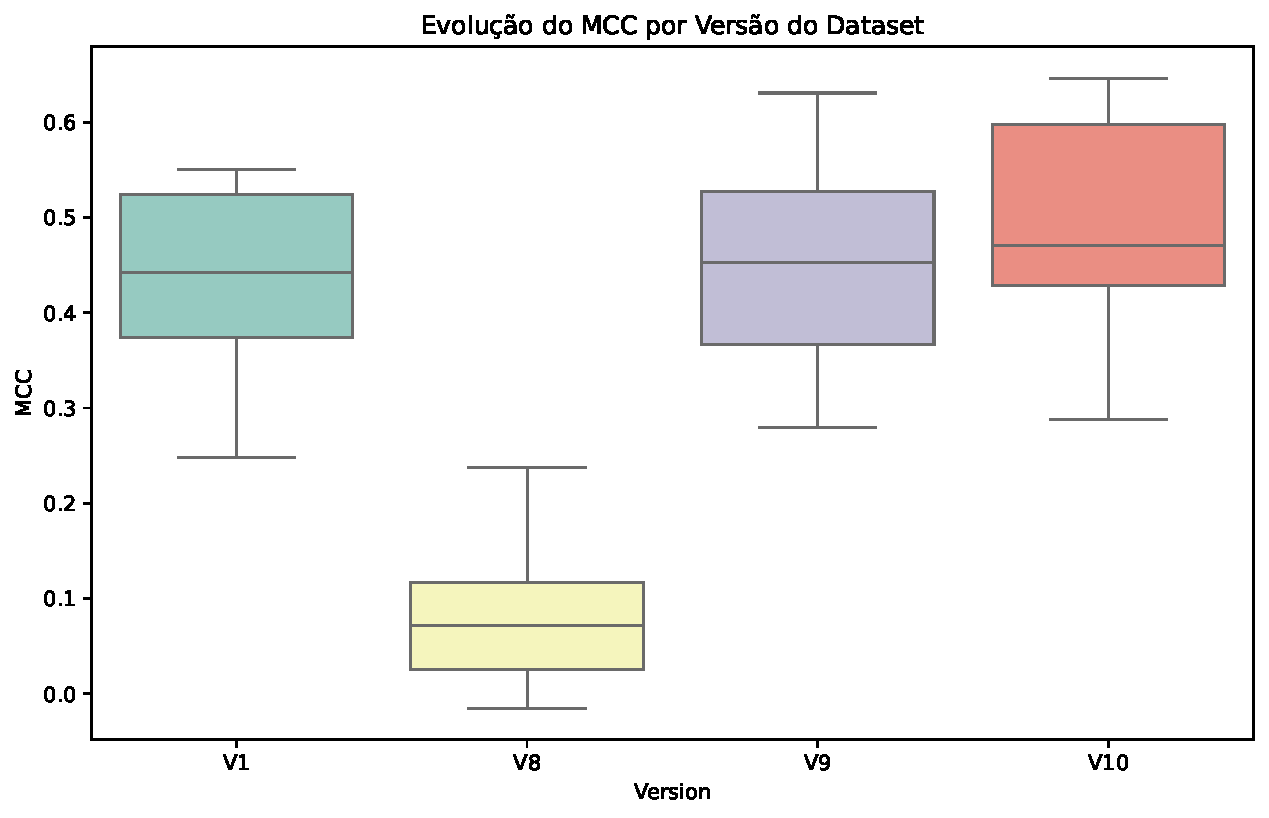
\includegraphics[width=0.8\textwidth]{images/linear_evolution_mcc.pdf}
  \caption{Evolução do MCC por versão do dataset. O salto de performance na V10 justifica sua seleção para as análises subsequentes.}
  \label{fig:linear_evolution}
\end{figure}

Para validar se essa diferença entre as versões é estatisticamente relevante, aplicou-se o teste de \textbf{Friedman}, complementado pelo teste \textit{post-hoc} de Wilcoxon com correção de Bonferroni. A Tabela \ref{tab:friedman_detailed} apresenta os postos médios e os grupos de significância.

\begin{table}[!h]
    \centering
    \begin{threeparttable}
    \caption{Resultado detalhado do teste de Friedman e grupos de significância.}
    \label{tab:friedman_detailed}
    \begin{tabular}{lrc}
\toprule
\textbf{Versão do Dataset} & \textbf{Posto Médio} & \textbf{Grupo} \\
\midrule
V10 & 1.25 & (a) \\
V9 & 2.12 & (a) \\
V1 & 2.62 & (a) \\
V8 & 4.00 & (c) \\
\midrule
\multicolumn{3}{l}{\textbf{Estatística de Friedman}: $\chi^2 = 19.05$ ($p = 2.67e-04$)} \\
\multicolumn{3}{l}{\small Grupos com mesma letra não apresentam diferença estatística ($p > 0,05$)} \\
\bottomrule
\end{tabular}
    \begin{tablenotes}
            \small 
            \item[] Fonte: Do autor.
        \end{tablenotes}
        \end{threeparttable}
\end{table}

A Figura \ref{fig:critical_difference} apresenta o diagrama de \textbf{Diferença Crítica (CD)}. O diagrama permite visualizar que a versão \textbf{V10} (Posto Médio 1.12) e a versão \textbf{V9} (Posto Médio 1.88) pertencem ao mesmo grupo de significância, sendo ambas estatisticamente superiores ao baseline (V1) e à versão experimental V8. 

\begin{figure}[h!]
  \centering
  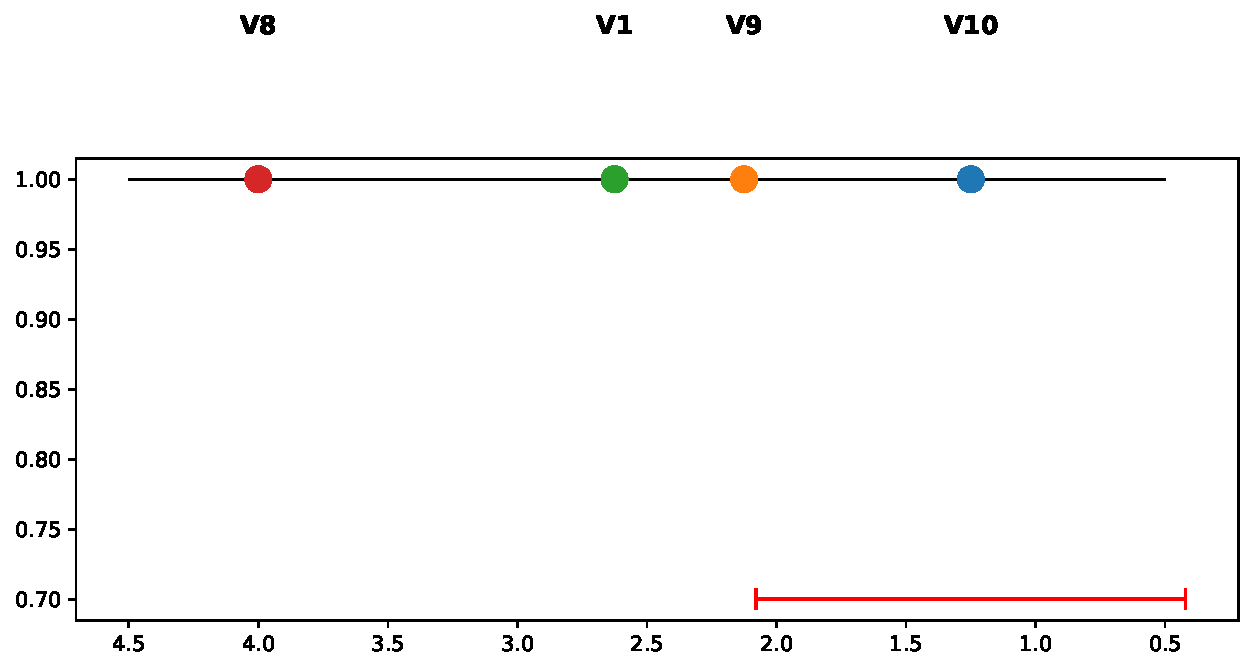
\includegraphics[width=0.9\textwidth]{images/critical_difference_friedman.pdf}
  \caption{Diagrama de Diferença Crítica (CD) entre as versões do dataset. Versões à esquerda apresentam melhor ranqueamento. A barra vermelha indica a distância mínima para que a diferença seja estatisticamente significativa.}
  \label{fig:critical_difference}
\end{figure}

Embora a V10 e a V9 sejam estatisticamente similares em termos de ranking global, a \textbf{V10} obteve o maior MCC absoluto entre todos os experimentos. Portanto, ela foi selecionada como o dataset padrão para as validações de hipóteses arquiteturais ($H_1$) e de eficiência industrial ($H_4$).
